
\documentclass[12pt, a4paper]{report}
\usepackage{epsfig}
\usepackage{subfigure}
%\usepackage{amscd}
\usepackage{amssymb}
\usepackage{graphicx}
%\usepackage{amscd}
\usepackage{amssymb}
\usepackage{subfiles}
\usepackage{framed}
\usepackage{subfiles}
\usepackage{amsthm, amsmath}
\usepackage{amsbsy}
\usepackage{framed}
\usepackage[usenames]{color}
\usepackage{listings}
\lstset{% general command to set parameter(s)
	basicstyle=\small, % print whole listing small
	keywordstyle=\color{red}\itshape,
	% underlined bold black keywords
	commentstyle=\color{blue}, % white comments
	stringstyle=\ttfamily, % typewriter type for strings
	showstringspaces=false,
	numbers=left, numberstyle=\tiny, stepnumber=1, numbersep=5pt, %
	frame=shadowbox,
	rulesepcolor=\color{black},
	,columns=fullflexible
} %
%\usepackage[dvips]{graphicx}
\usepackage{natbib}
\bibliographystyle{chicago}
\usepackage{vmargin}
% left top textwidth textheight headheight
% headsep footheight footskip
\setmargins{3.0cm}{2.5cm}{15.5 cm}{22cm}{0.5cm}{0cm}{1cm}{1cm}
\renewcommand{\baselinestretch}{1.5}
\pagenumbering{arabic}
\theoremstyle{plain}
\newtheorem{theorem}{Theorem}[section]
\newtheorem{corollary}[theorem]{Corollary}
\newtheorem{ill}[theorem]{Example}
\newtheorem{lemma}[theorem]{Lemma}
\newtheorem{proposition}[theorem]{Proposition}
\newtheorem{conjecture}[theorem]{Conjecture}
\newtheorem{axiom}{Axiom}
\theoremstyle{definition}
\newtheorem{definition}{Definition}[section]
\newtheorem{notation}{Notation}
\theoremstyle{remark}
\newtheorem{remark}{Remark}[section]
\newtheorem{example}{Example}[section]
\renewcommand{\thenotation}{}
\renewcommand{\thetable}{\thesection.\arabic{table}}
\renewcommand{\thefigure}{\thesection.\arabic{figure}}
\title{Research notes: linear mixed effects models}
\author{ } \date{ }


\begin{document}
	\author{Kevin O'Brien}
	\title{Mixed Models for Method Comparison Studies}
	\tableofcontents
	
	%----------------------------------------------------------------------------------------%
	\newpage
%	Quick Introduction to Residuals
%	Assumptions Concerning Residuals
%	Residals for LME models
%	Conditional and Marginal Residuals
	
	\section{Validating Models with Residuals}
	%http://www.itl.nist.gov/div898/handbook/pmd/section4/pmd44.htm
	Model validation is possibly the most important step in the model building sequence. It is also one of the most overlooked. Often the validation of a model seems to consist of nothing more than quoting the $R^2$ statistic from the fit (which measures the fraction of the total variability in the response that is accounted for by the model). Unfortunately, a high $R^2$ value does not guarantee that the model fits the data well. Use of a model that does not fit the data well will not provide any meaningful insights to the underlying research questions.
	
	\subsubsection{Residual Analysis}
	A residual is the difference between an observed quantity and its estimated or predicted value. Residuals are used to examine model assumptions and to detect outliers and potentially influential data	point. 
	
	Residual analysis is a widely used model validation technique. A residual is simply the difference between an observed value and the corresponding fitted value, as predicted by the model. The rationale is that, if the model is properly fitted to the model, then the residuals would approximate the random errors that one should expect.
	that is to say, if the residuals behave randomly, with no discernible trend, the model has fitted the data well. If some sort of non-random trend is evident in the model, then the model can be considered to be poorly fitted.
		
			Statistical software environments, such as the \texttt{R} Programming language, provides a suite of tests and graphical procedures for appraising a fitted linear model, with several 
			of these procedures analysing the model residuals.
			
			In classical linear models, model diagnostics techniques determine whether or not the distributional assumptions are satisfied, and to assess the influence of unusual observations, and have been become a required part of any statistical analysis. Well established methods are commonly available in statistical packages and standard textbooks on applied regression. However it has been noted by several papers that model diagnostics do not often accompany LME model analyses. \citet{schabenberger} discusses the state of LME diagnostics tools, providing a useful summary of established measures.
			
			%\subsubsection{Model Data Agreement} %1.1.1
			\citet{schabenberger} describes the examination of model-data agreement as comprising several elements; residual analysis, goodness of fit, collinearity diagnostics and influence analysis.
			
			
			In classical linear models, an examination of model-data agreement has traditionally revolved around
			
			The second part of the chapter looks at diagnostics techniques for LME models, firsly covering the theory, then proceeding to a discussion on 
			implementing these using \texttt{R} code.
			
			While a substantial body of work has been developed in this area, there is still areas worth exploring. 
			In particular the development of graphical techniques pertinent to LME models should be looked at.
			
	
			
	
		
		For classical linear models, residual diagnostics are typically implemented as a plot of the observed residuals and the predicted values. A visual inspection for the presence of trends inform the analyst on the validity of distributional assumptions, and to detect outliers and influential observations. Statistical software environments, such as the \texttt{R} programming language, provides a suite of tests and graphical procedures for appraising a fitted linear model, with several 
		of these procedures analysing the model residuals.
		
	
	
	
	
	
	%% \subsubsection{Why Use Residuals?}
	%If the model fit to the data were correct, the residuals would approximate the random errors that make the relationship between the explanatory variables and the response variable a statistical relationship. Therefore, if the residuals appear to behave randomly, it suggests that the model fits the data well. On the other hand, if non-random structure is evident in the residuals, it is a clear sign that the model fits the data poorly. The subsections listed below detail the types of plots to use to test different aspects of a model and give guidance on the correct interpretations of different results that could be observed for each type of plot.
	%------------------------------------------------------------------------------------------------------------------------ %
	\subsubsection{Introduction to Residual Analysis}

	
	However, for LME models the matter of residual is more complex, both from a theoretical point of view and from the practical matter of implementing a comprehensive analysis using statistical software. As the LME model can be tailored to the needs of the particular research question, the rationale behind the model appraisal must follow accordingly.
	
	
	%===================================================================================================%
	
	\subsection*{Preliminary Residual Analysis }
	
	% This short section will look at residual analysis for LME models. 
	The underlying assumptions for LME models are similar to those of classical linear mdoels. There are two key techniques: a residual plot and the normal probability plot. Using the nlme package it is possible to create plots specific to each method. This is useful in determine which methods `disagree` with the rest.
	Analysis of the residuals would determine if the methods of measurement disagree systematically, or whether or not erroneous measurements associated with a subset of the cases are the cause of disagreement.
	Erroneous measurements are incorrect measurements that indicate disagreement between methods that would otherwise be in agreement.
	%======================================================== %
	Once the residuals are computed, they can be used to make an assessment about the model fit. For the LME model described in Chapter 2, we can plot the residuals against the fitted values, to assess the assumption of constant variance. f the points in a residual plot are randomly dispersed around the horizontal axis, a linear regression model is appropriate for the data; otherwise, a non-linear model is more appropriate.
	
	%	\begin{figure}[h!]
	%		\centering
	%		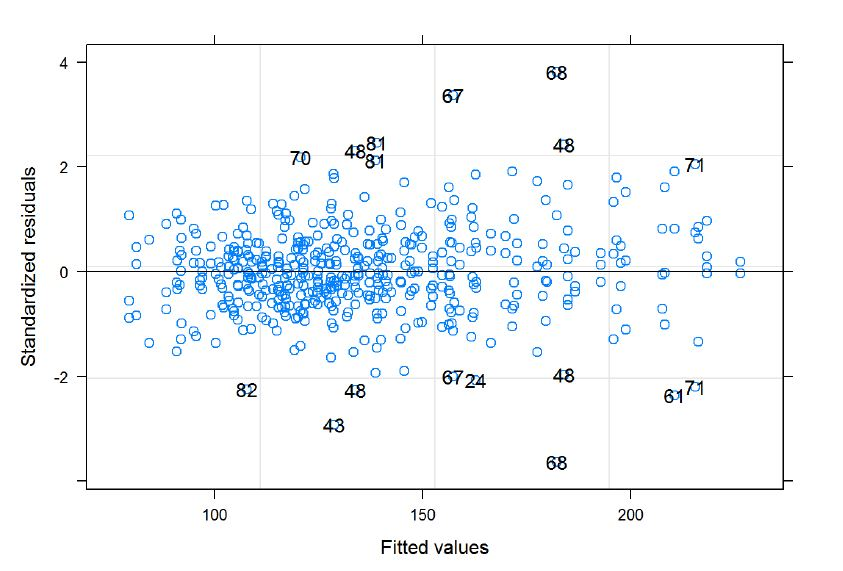
\includegraphics[width=0.9\linewidth]{images/Residuals-JS-Roy}
	%		\caption{}
	%		\label{fig:Residuals-JS-Roy}
	%	\end{figure}
	
	LME models assume that the residuals of the model are normally distributed.  The residuals can be divided according to groups according to the method of measurement. In the following examples, we seperately assess normality the \textit{J} method residuals (the first 255 residuals) and \textit{S} method residuals (the remaining 255). Importantly the residuals from the \textit{J} method are normally distributed, but there is non-normality of the residuals according to the \textit{S} method.
	
	%===================================================================================================%
	
	
	Normal probability plots can be rendered for each level of the random effects.  LME models assume that not only the within-cluster residuals are normally distributed, but that each level of the random effects are as well. % 
	
	%
	%\subsubsection{Introduction}
	%In statistics and optimization, statistical errors and residuals are two closely related and easily confused measures of the deviation of an observed value of an element of a statistical sample from its "theoretical value". The error (or disturbance) of an observed value is the deviation of the observed value from the (unobservable) true function value, while the residual of an observed value is the difference between the observed value and the estimated function value.
	%
	%The distinction is most important in regression analysis, where it leads to the concept of studentized residuals.
	%
	%
	
	
	
	
	
	
	
	
	
	%---------------------------------------------------------------------------%
	
	
	
	
	
	
	
	\subsubsection{Residual Plots}
	A residual plot is a graph that shows the residuals on the vertical axis and the independent variable on the horizontal axis. If the points in a residual plot are randomly dispersed around the horizontal axis, a linear regression model is appropriate for the data; otherwise, a non-linear model is more appropriate.
	
	%		\begin{framed}
	%			\begin{verbatim}
	%			par(mfrow=c(1,2))
	%			qqnorm((resid(JS.roy1)[1:255]),
	%			pch="*",col="red",
	%			ylim=c(-40,40),
	%			main="Method J")
	%			qqline(resid(JS.roy1)[1:255],col="blue")
	%			qqnorm((resid(JS.roy1)[256:510]),
	%			pch="*",col="red",
	%			ylim=c(-40,40),
	%			main="Method S")
	%			qqline(resid(JS.roy1)[256:510],col="blue")
	%			par(mfrow=c(1,1))
	%			\end{verbatim}	
	%		\end{framed}
	
	
	\begin{figure}[h!]
		\centering
		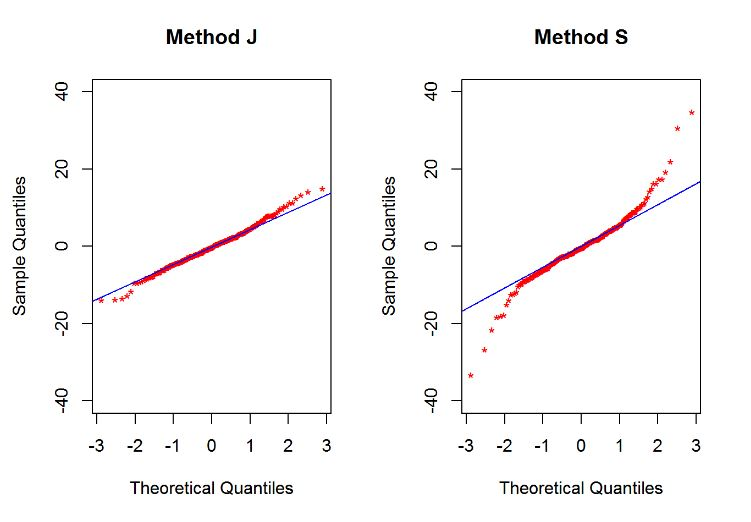
\includegraphics[width=1.1\linewidth]{images/Resid-newplot2}
		\caption{}
		\label{fig:Resid-newplot2}
	\end{figure}
	
	
	\begin{figure}[h!]
		\centering
		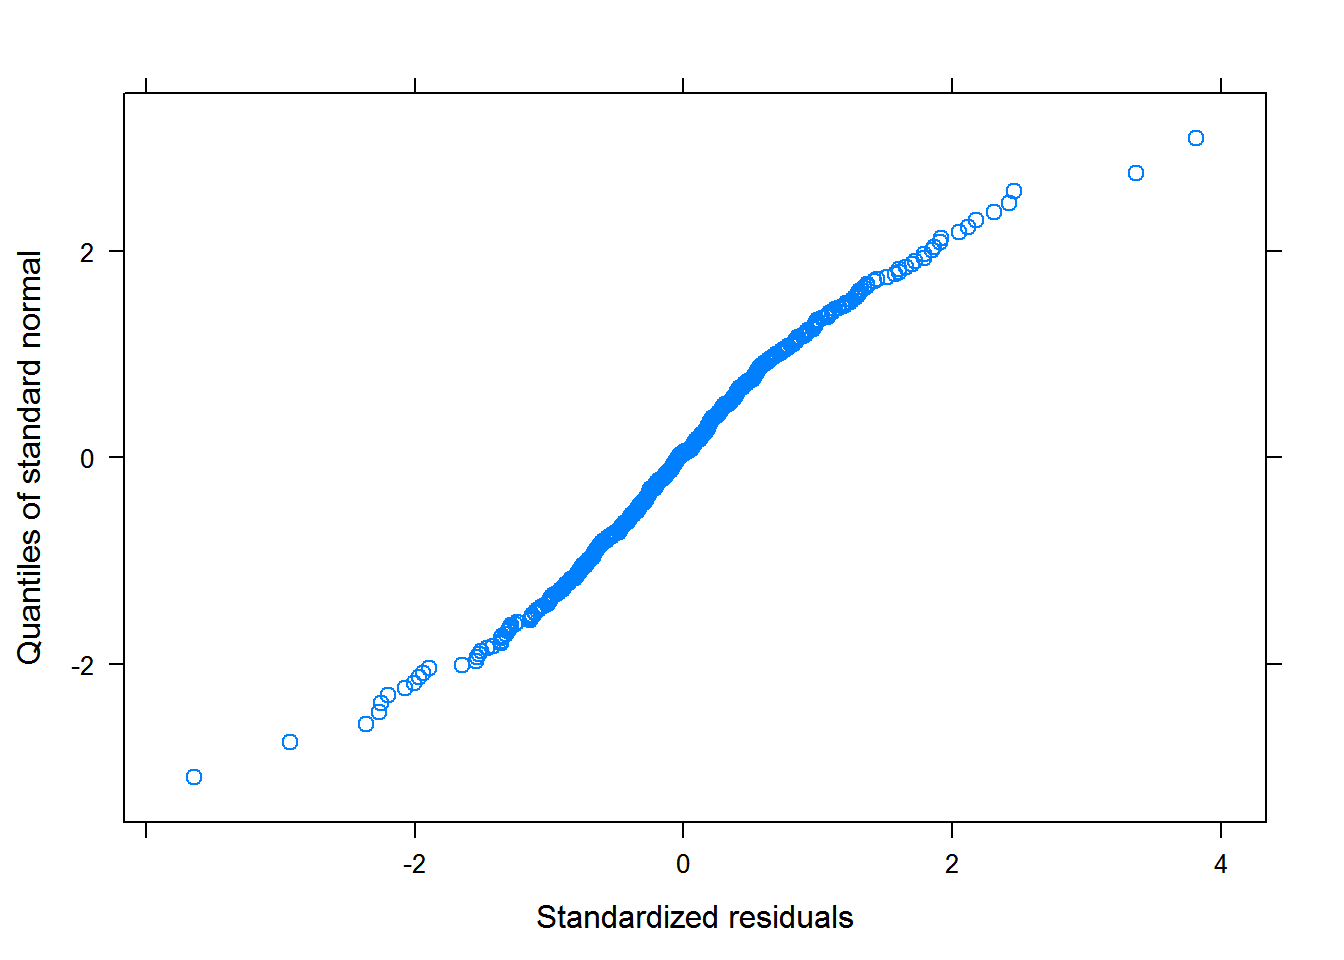
\includegraphics[width=0.9\linewidth]{images/ResidPlot3}
		\label{fig:ResidPlot3}
	\end{figure}
	

	\begin{figure}[h!]
		\centering
		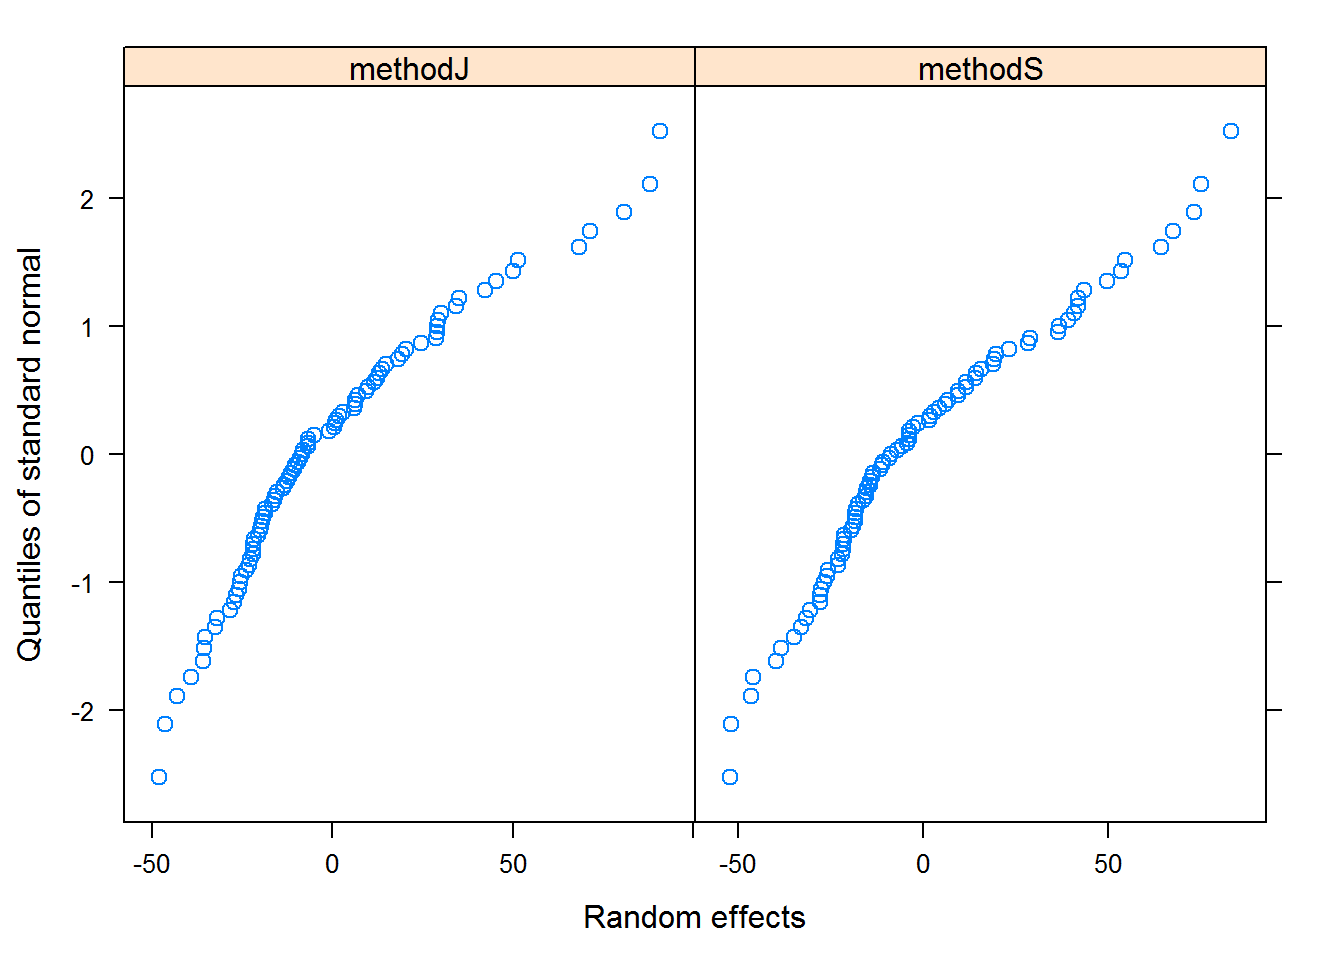
\includegraphics[width=0.9\linewidth]{images/ResidPlot2}
		\caption{}
		\label{fig:ResidPlot2}
	\end{figure}
	
	%--Marginal and Conditional Residuals
	
	
	
	

	\subsection{Residual diagnostics} %1.3
	
	
	For an LME model, the \textit{raw} residuals at level $i$ are obtained by subtracting the fitted levels at that level from the response vector If we require a \textit{Pearson} type residual, we further dviide this by the estimated within-group standard error. The Pearson residual is the raw residual divided by the square root of the the within-group standard error for both methods. The fitted values at level $i$ are obtained by adding together the population fitted values (based only on the fixed effects estimates) and the estimated contributions of the random effects to the fitted values at grouping levels less or equal to $i$. In addition to Raw and Pearson residuals, there are normalized residuals : standardized residuals pre-multiplied by the inverse square-root factor of the estimated error correlation matrix. For the forthcoming examples, we will use the raw residuals.
		\subsubsection{Pearson Residual}%1.4.5
		
		Another possible scaled residual is the \index{Pearson residual} `Pearson residual', whereby a residual is divided by the standard deviation of the dependent variable. The Pearson residual can be used when the variability of $\hat{\beta}$ is disregarded in the underlying assumptions.
	\newpage
	For an lme object, the residuals at level $i$ are obtained by subtracting the fitted levels at that level from the response vector (and dividing by the estimated within-group standard error, if \texttt{type="pearson"}).The Pearson residual is the raw residual divided by the square root of the variance function (here, the Within-group standard error for both methods, 6.11 and 9.11 respectively). The fitted values at level $i$ are obtained by adding together the population fitted values (based only on the fixed effects estimates) and the estimated contributions of the random effects to the fitted values at grouping levels less or equal to $i$.
		
		\begin{description}
			\item["\texttt{response}"]: the “raw” residuals (\textit{observed - fitted}) are used. This is the default option.
			\item["\texttt{pearson}"]: the standardized residuals (raw residuals divided by the corresponding standard errors) are used; 
			\item["\texttt{normalized}"]: the normalized residuals (standardized residuals pre-multiplied by the inverse square-root factor of the estimated error correlation matrix) are used.
		\end{description}
	%-----------------------------------------------------------------------------------------%
	\subsection*{Residuals}
	
	\begin{description}
		\item[residuals.lme] 
		The residuals at level $i$ are obtained by subtracting the fitted levels at that level from the response
		vector (and dividing by the estimated within-group standard error, if \texttt{type="pearson")}. The fitted
		values at level $i$ are obtained by adding together the population fitted values (based only on the
		fixed effects estimates) and the estimated contributions of the random effects to the fitted values at
		grouping levels less or equal to $i$.
	\end{description}
	

	\subsection{Distinction From Linear Models (Schabenberger page 3)}
	%% Where is this coming from?
	%% 
	The differences between perturbation and residual analysis in the linear model and the linear mixed model
	are connected to the important facts that b and b
	depend on the estimates of the covariance parameters,
	that b has the form of an (estimated) generalized least squares (GLS) estimator, and that 
	is a random
	vector.
	In a mixed model, you can consider the data in a conditional and an unconditional sense. If you imagine
	a particular realization of the random effects, then you are considering the conditional distribution
	Y|
	If you are interested in quantities averaged over all possible values of the random effects, then
	you are interested in Y; this is called the marginal formulation. In a clinical trial, for example, you
	may be interested in drug efficacy for a particular patient. If random effects vary by patient, that is a
	conditional problem. If you are interested in the drug efficacy in the population of all patients, you are
	using a marginal formulation. Correspondingly, there will be conditional and marginal residuals, for
	example.
	The estimates of the fixed effects  depend on the estimates of the covariance parameters. If you are
	interested in determining the influence of an observation on the analysis, you must determine whether
	this is influence on the fixed effects for a given value of the covariance parameters, influence on the
	covariance parameters, or influence on both.
	Mixed models are often used to analyze repeated measures and longitudinal data. The natural experimental
	or sampling unit in those studies is the entity that is repeatedly observed, rather than each
	individual repeated observation. For example, you may be analyzing monthly purchase records by
	customer. 
	An influential “data point” is then not necessarily a single purchase. You are probably more
	interested in determining the influential customer. This requires that you can measure the influence
	of sets of observations on the analysis, not just influence of individual observations.
	%		\item The computation of case deletion diagnostics in the classical model is made simple by the fact that
	%		%estimates of  and 2, which exclude the ith observation, can be %computed without re-fitting the
	%		model. Such update formulas are available in the mixed model only if you assume that the covariance
	%		parameters are not affected by the removal of the observation in question. This is rarely a reasonable
	%		assumption.
	The application of well-known concepts in model-data diagnostics to the mixed model can produce results
	that are at first counter-intuitive, since our understanding is steeped in the ordinary least squares
	(OLS) framework. As a consequence, we need to revisit these important concepts, ask whether they
	are “portable” to the mixed model, and gain new appreciation for their changed properties. An important
	example is the ostensibly simple concept of leverage. 
	%		\item The definition of leverage adopted by
	%		the MIXED procedure can, in some instances, produce negative values, which are mathematically
	%		impossible in OLS. Other measures that have been proposed may be non-negative, but trade other
	%		advantages. Another example are properties of residuals. While OLS residuals necessarily sum to
	%		zero in any model (with intercept), this not true of the residuals in many mixed models.
	
	
	\subsubsection{Studentized Residuals}
	Standardization is not possible in practice. Studentized residuals are residuals divided by the estimated standard estimation.
	[Gregoire,Schabenberger, Barrett (1995)]
	
	\[\boldsymbol{r}_{m} = \boldsymbol{Y} -  \boldsymbol{X} \boldsymbol{\hat{\beta}} \]
	
	\[\boldsymbol{r}_{c} = \boldsymbol{Y} -  \boldsymbol{X} \boldsymbol{\hat{\beta}} -  \boldsymbol{Z} \boldsymbol{\hat{\gamma}}\]
	
	For the individual observation the raw studentized and pearson type residuals are computed as follows:
	\[r_{mi} =Y_{i} -X^{\prime} \boldsymbol{\hat{\beta}}\]
	
	\[r_{ci} = r_{mi} - Y_{i} - z_{i}^{\prime} \boldsymbol{\hat{\gamma}}\]
	
	

	\subsection{Taxonomy of LME Residuals}
	A residual is the difference between an observed quantity and its estimated or predicted value. 
	
	Standard residual and influence diagnostics for linear models can
	be extended to linear mixed models. The dependence of
	fixed-effects solutions on the covariance parameter estimates has
	important ramifications in perturbation analysis. To gauge the
	full impact of a set of observations on the analysis, covariance
	parameters need to be updated, which requires refitting of the
	model.
	%---http://www.stat.purdue.edu/~bacraig/notes598S/SUGI_Paper_Schabenberger.pdf
	
	In LME models, there are two types
	of residuals, marginal residuals and conditional residuals. 
	For LME models, \citet{schab} describes two types of residuals, marginal residuals and conditional residuals. 
	
	\begin{itemize}
		\item A marginal residual is the difference between the observed data and the estimated (marginal) mean, $r_{mi} = y_i - x_0^{\prime} \hat{b}$
		\item A conditional residual is the difference between the observed data and the predicted value of the observation,
		$r_{ci} = y_i - x_i^{\prime} \hat{b} - z_i^{\prime} \hat{\gamma}$	
	\end{itemize} 
	In a model without random effects, both sets of
	residuals coincide \citep{schabenberger}. We shall revert to this matter in due course.
	
	
	
	
	
	The definitions of both marginal residuals ($r_m$) and conditional residuals ($r_c$) follow from the definitions of marginal and conditional means in the LME model 
	$E[\boldsymbol{Y}] = \boldsymbol{X}\boldsymbol{\beta}$ and $E[\boldsymbol{Y|\boldsymbol{u}}] = \boldsymbol{X}\boldsymbol{\beta} + \boldsymbol{Z}\boldsymbol{u}$, respectively.
	
	A marginal residual is the difference between the observed data and the estimated marginal mean. A conditional residual is the difference between the observed data and the predicted value of the observation. In a model without random effects, both sets of	residuals coincide.
	
	
	The conditional (subject-specific) and marginal (population-averaged) formulations in the linear mixed model enable you to consider conditional residuals that use the estimated BLUPs of the random effects, and marginal residuals which are deviations from the overall mean. Residuals using the BLUPs are useful to diagnose whether the random effects components
	in the model are specified correctly, marginal residuals are useful to diagnose the fixed-effects components.	
	
	
	The raw residuals $r_{mi}$ and $r_{ci}$ are usually not well suited for these purposes.
	
	\begin{itemize}
		\item Conditional Residuals $r_{ci}$
		\item Marginal Residuals $r_{mi}$
	\end{itemize}
	
	
	\citet{pb} describes three types of residual that describe the variabilities
	present in LME models
	\begin{enumerate}
		\item marginal residuals, $\hat{\xi}$, which predict marginal errors,
		\item conditional residuals, $\hat{\epsilon}$, which predict conditional errors,
		\item the BLUP,$\boldsymbol{Z\hat{b}}$, that predicts random effects.
	\end{enumerate}
	Each type of residual is useful to evaluates some assumption of the model.
	
	%- http://www.ime.usp.br/~jmsinger/MAE5705/EMR2013.pdf
	
	According to Hilton \& Minton (1995), a residual is considered pure for a specfic type fo error
	if it depends only on the fixed components and on the error that it is supposed to predict.
	Residuals that depend on other types of error are known as `confounded errors'.
	
	
	
	
	\subsubsection{Conditional and Marginal Residuals}
	Conditional residuals include contributions from both fixed and random effects, whereas marginal residuals include contribution from only fixed effects.
	
	Suppose the linear mixed-effects model lme has an $n \times p$ fixed-effects design matrix $\boldsymbol{X}$ and an $n \times q$ random-effects design matrix $\boldsymbol{Z}$. 
	
	Also, suppose the p-by-1 estimated fixed-effects vector is $\hat{\beta}$ , and the q-by-1 estimated best linear unbiased predictor (BLUP) 
	vector of random effects is $\hat{b}$ . The fitted conditional response is
	
	\[ \hat{y}_{Cond} = X \hat{\beta} + Z \hat{b} \]
	
	and the fitted marginal response is
	
	
	\[ \hat{y}_{Mar} = X \hat{\beta} \]
	
	\subsubsection{Marginal Residuals}
	The marginal residuals are defined according to
	\begin{eqnarray*}
		\hat{\xi} = y - X\hat{\beta} = M^{-1}Qy. \\\nonumber
	\end{eqnarray*}
	
	
	%------------------------------------------------------------Section 4.2---%
	\subsubsection{Conditional Residuals}
	A conditional probability is the difference between the observed value and the predicted value of the dependent variable.
	\begin{equation*}
	\hat{\epsilon}_{i} = y_{i} - X_{i}\hat{\beta} + Z_{i}\hat{b}_{i}
	\end{equation*}
	
	In general conditional residuals are not well suited for verifying model assumptions and detecting outliers. Even if the true model residuals are uncorrelated and have equal variance, conditional variances will tend to be correlated and their variances may be different for different subgroups of individuals \citep{west}.
	
	
	
	
	For any type, you can compute the conditional or the marginal residuals. For example, the conditional raw residual is
	
	
	\[ r_{Cond} = y - X \hat{\beta} - Z \hat{b} \]
	
	and the marginal raw residual is
	
	
	
	\[ r_{Mar} = y - X \hat{\beta} \]
	
	
	
	
	In linear mixed effects models, diagnostic techniques may consider `conditional' residuals. A conditional residual is the difference between an observed value $y_{i}$ and the conditional predicted value $\hat{y}_{i} $.
	
	\[ \hat{\epsilon}_{i} = y_{i} - \hat{y}_{i} = y_{i} - ( X_{i}\hat{\beta} + Z_{i}\hat{b}_{i}) \]
	
	However, using conditional residuals for diagnostics presents difficulties, as they tend to be correlated and their variances may be different for different subgroups, which can lead to erroneous conclusions.
	
	%========================================================%
	
	% https://v8doc.sas.com/sashtml/insight/chap39/sect55.htm
	
	
	
	
	
	The \textbf{deviance residual} is the measure of deviance contributed from each observation and is given by
	\[r_{Di} = \textrm{sign}( r_{i})
	\sqrt{ d_{i}}\]
	where $d_i$ is the individual deviance contribution.
	The deviance residuals can be used to check the model fit at each observation for generalized linear models. 
	
	%These residuals are stored in variables named \textit{RD\_yname} for each response variable, where yname is the response variable name. 
	
	The standardized and studentized deviance residuals are
	\[
	r_{Dsi} = \frac{r_{Di}}{\sqrt{\hat{ \phi} (1- h_{i})} }\]
	\[r_{Dti} = \frac{r_{Di}}{\sqrt{ \hat{ \phi}_{(i)}
			(1- h_{i})}}\]
	
	
	
	%-------------------------------------------------------------- %
	\subsubsection*{Residuals}
	Studentized residuals, error contrast matrices and the inverse of the response variance covariance matrix are regular components of these tools.

	
	%---------------------------------------------------------------------------%
	
	
	

	\subsubsection{Residual variance}
	When $\sigma^2$ is profiled out of the marginal variance-covariance matrix, a closed-form estimate of $\sigma^2$ that is only based on only the remaining observation
	an be computed as follows, provided $\boldsymbol{V} = \boldsymbol{V}(\boldsymbol{\theta}) $
	[cite: Hurtado 1993]

	\subsubsection{Reduced Data Set}
	It is important to determine if a specific group of cases or subjects give rise to the lack of agreement in the methods. If one were to examine fitted model if these cases were removed.
	
	%\begin{framed}
	%	\begin{verbatim}
	%	
	%	blood.red <- blood[!(blood$subject %in% c(68,78,80)),]
	%	dim(blood.red)
	%	# 27 observations should be removed.
	%	
	%	blood.NLME.red <-lme(BP ~ method-1 , random=~1|subject,data = blood.red)
	%	plot(blood.NLME.red, resid(., type = "p") ~ fitted(.) | method, abline = 0, id=.05)
	%	\end{verbatim}
	%\end{framed}
	
	In this instance, we conclude that there is a systemic diagreement between method S and the other two methods, and that lack of agreement can not be sourced to a handful of cases.
	\begin{figure}[h!]
		\centering
		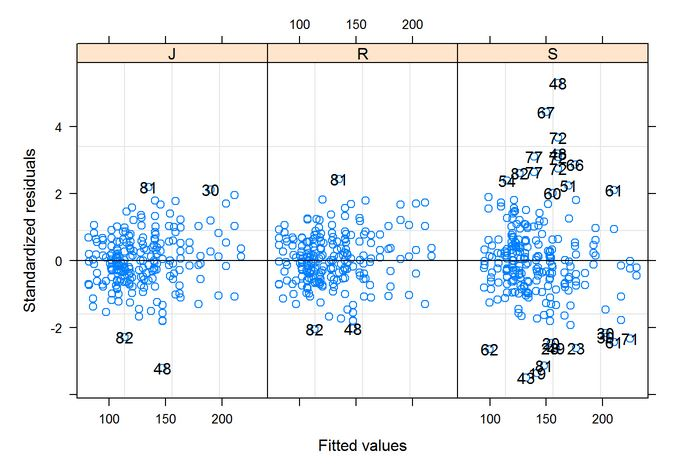
\includegraphics[width=0.7\linewidth]{images/bloodnlmeResidPlot2B}
	\end{figure}
	 
	 \newpage
	
	
		
	

	\subsection{Standardization and Studentization} %1.4.2
	To alleviate the problem caused by inconstant variance, the residuals can be scaled (i.e. divided) by their standard deviations. This results in a \index{standardized residual}`standardized residual'. A random variable is said to be standardized if the difference from its mean is scaled by its standard deviation. The residuals  have mean zero but their variance is unknown, it depends on the true values of $\theta$. Standardization is  not possible in practice. Because true standard deviations are frequently unknown, one can instead divide a residual by the estimated standard deviation to obtain the \index{studentized residual}`studentized residual. 
	%Instead, you can compute studentized residuals by dividing a residual by an estimate of its standard deviation. 
	If that estimate is independent of the $i-$th observation, the process is termed \index{external studentization}`external studentization'. This is usually accomplished by excluding the $i-$th observation when computing the estimate of its standard error. If the observation contributes to the
	standard error computation, the residual is said to be \index{internally studentization}internally studentized.
	Externally \index{studentized residual} studentized residual require iterative influence analysis or a profiled residuals variance \textbf{(CITE)}.
	
	
	% \subsubsection{Computation}%1.4.4
	
	The computation of internally studentized residuals relies on the diagonal entries of $\boldsymbol{V} (\hat{\theta})$ - $\boldsymbol{Q} (\hat{\theta})$, where $\boldsymbol{Q} (\hat{\theta})$ is computed as
	
	\[ \boldsymbol{Q} (\hat{\theta}) = \boldsymbol{X} ( \boldsymbol{X}^{\prime}\boldsymbol{Q} (\hat{\theta})^{-1}\boldsymbol{X})\boldsymbol{X}^{-1} \]
	
	

	
	
	
	
	%-----------------------------------------------------------------------------------------%
	In this chapter, we will look at residual analysis and diagnostic toold for LME models, and discuss how they can be applied to the Method Comparison Problem.	In classical linear models, a residual is the difference between an observed value and its estimated or predicted value. For LME models, the topic is more complicated, and still a matter of active research. 
	
	
	\subsubsection{Internally and Externally Studentized Residuals}
	%Internally and Externally Studentized Residuals
	The computation of internally studentized residuals relies on the diagonal values of $\boldsymbol{V(\hat{\theta})} - \boldsymbol{Q(\hat{\theta})}$
	Externally studentized residuals require iterative influece analysis or a profiled residual variance.
	
	Cook's Distance
	\[ \boldsymbol{\delta}_{(U)} = \boldsymbol{\hat{\beta}}  - \boldsymbol{\hat{\beta}}_{(U)} \]
	A DFFIT measures the change in predicted values due to the removal of data points.
	(Belsey, Kuh and Welsch (1980))
	%[ \mbox{DFFITS}_{i} = \frac{\hat{y}_i - \hat{y}_{i(U)}}{ese(\hat{y}_i)} \]
	
	$\boldsymbol{D(\beta)}  = \boldsymbol{\delta}^{\prime}_{(U)} \boldsymbol{\delta}_{(U)} / rank(\boldsymbol{X})$
	Cook's D can be calibrated according to a chi-square distribution with degress of freedom equal to the rank of $\boldsymbol{X}$ \citep{Christensen}.
	
	%	$ \mbox{CovTrace}(\boldsymbol{\beta})$
	
	
	%========================================================================================== %


	\subsection{Checking the Assumption by Method}
	
	
	

	\subsubsection{Diagnostic Plots for LME models}
	
	
	
	
	
	\begin{figure}[h!]
		\centering
		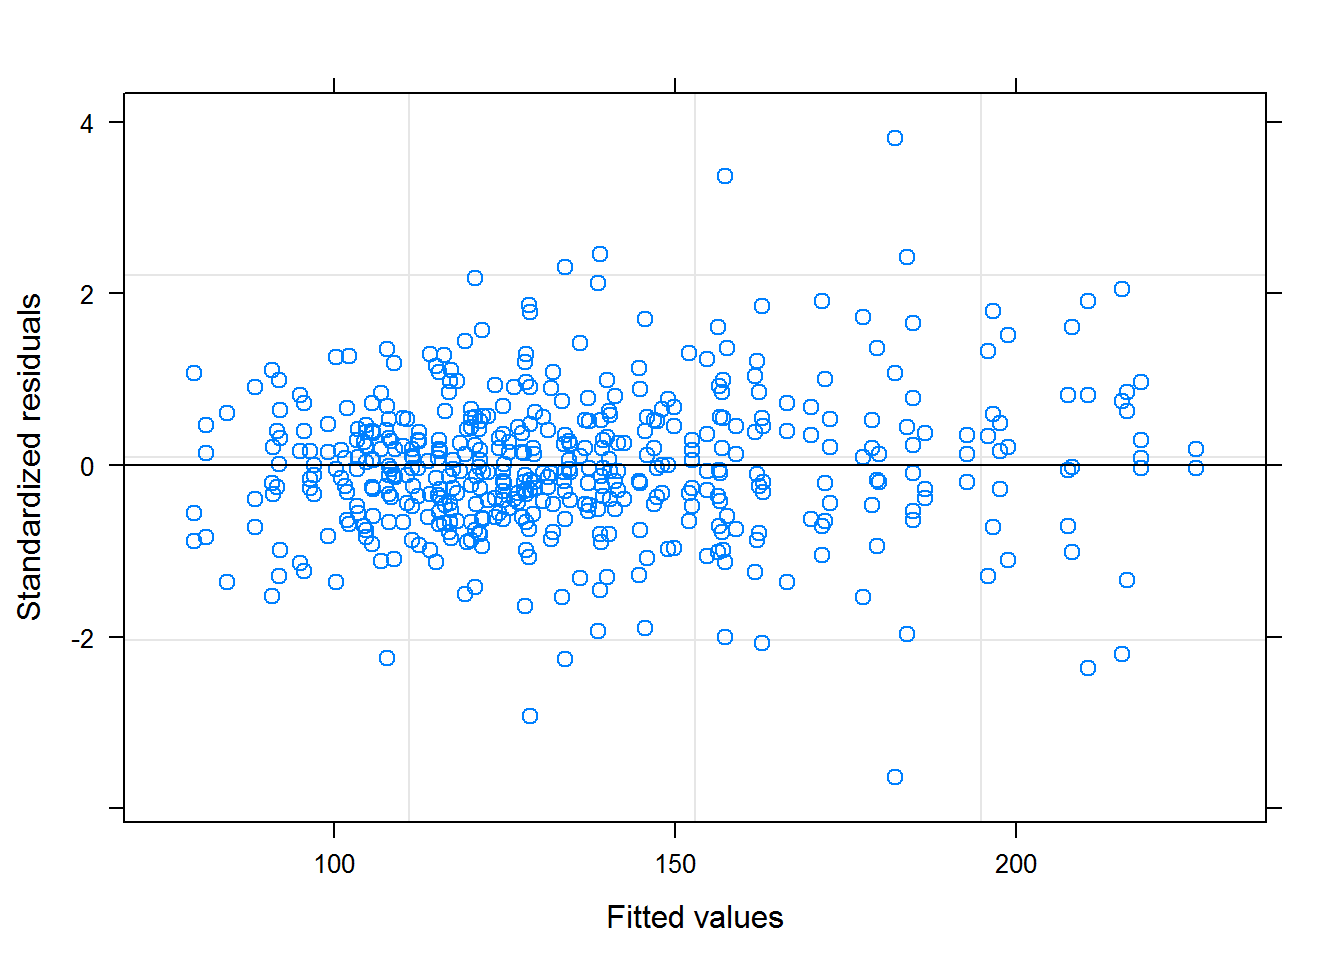
\includegraphics[width=0.9\linewidth]{images/ResidPlot1}
		\caption{}
		\label{fig:ResidPlot1}
	\end{figure}
	
	
	
	\begin{figure}[h!]
		\centering
		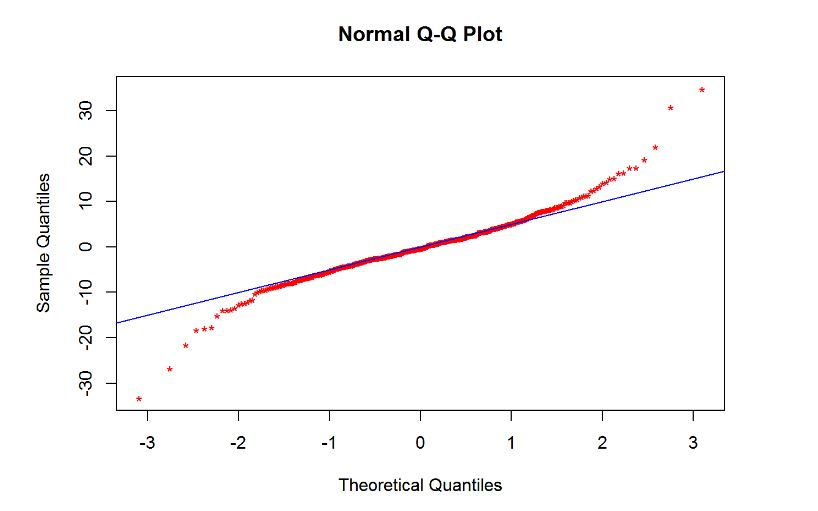
\includegraphics[width=0.7\linewidth]{images/Resid-newplot}
		\caption{}
		\label{fig:Resid-newplot}
	\end{figure}
	
	
	
	
	\subsubsection{Reduced Data Set}
	It is important to determine if a specific group of cases or subjects give rise to the lack of agreement in the methods. If one were to examine fitted model if these cases were removed.
	
	In this instance, we conclude that there is a systemic diagreement between method S and the other two methods, and that lack of agreement can not be sourced to a handful of cases.
	\begin{figure}[h!]
		\centering
		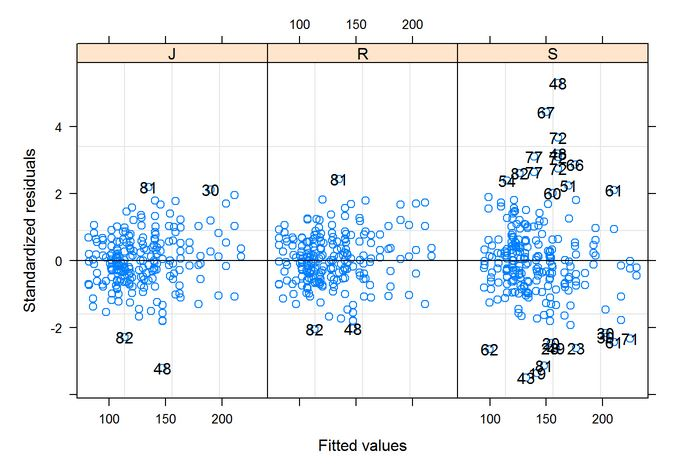
\includegraphics[width=0.7\linewidth]{images/bloodnlmeResidPlot2B}
	\end{figure}
	
	
	
	
	
	
	
	
	
	
	%\subsection{Introduction (Page 1)}
	%
	%Linear models for uncorrelated data have well established measures to gauge the influence of one or more
	%observations on the analysis. For such models, closed-form update expressions allow efficient computations
	%without refitting the model. 
	%
	%
	%When similar notions of statistical influence are applied to mixed models,
	%things are more complicated. Removing data points affects fixed effects and covariance parameter estimates.
	%Update formulas for “\textit{leave-one-out}” estimates typically fail to account for changes in covariance
	%parameters. 
	%
	%Moreover, in repeated measures or longitudinal studies, one is often interested in multivariate
	%influence, rather than the impact of isolated points. 
	
	% This paper examines extensions of influence measures
	% in linear mixed models and their implementation in the MIXED procedure.
	
	
	
	
	
	
	
	
	
	A marginal residual is the difference between the observed data and the estimated (marginal) mean, 
	\[r_{mi} = y_i - x_0^{\prime} \hat{b} =x^{T}_{i}\hat{\beta}\]
	
	\[y - X\beta = Z \eta +\epsilon \]
	
	A conditional residual is the difference between an observed value $y_{i}$ and the conditional predicted value $\hat{y}_{i} $,
	\[r_{ci} = y_i - x_i^{\prime} \hat{b} - z_i^{\prime} \hat{\gamma}\]
	
	\[y - X\beta - Z \eta = \epsilon \]
	 Marginal residuals are good for checking fixed effects.	
	 
	Conditional residuals include contributions from both fixed and random effects, whereas marginal residuals include contribution from only fixed effects. Marginal residuals should have mean of zero, but may show grouping structure. 
	Also they may not be homoscedastic.
	
	Plots of the elements of the marginal residual vector versus the explanatory variables in $X$ can be used to check the linearity of $\boldsymbol{y}$ in a similar manner to the residual plots used in linear models.
	Conditional residuals should have mean of zero with no grouping structure
	They should be homoscedastic. Conditional residuals are useful for checking normality of outliers
	
	%http://support.sas.com/documentation/cdl/en/statug/63033/HTML/default/viewer.htm#statug_mixed_sect024.htm
	
	In linear mixed effects models, diagnostic techniques may consider `conditional' residuals. A conditional residual is the difference between an observed value $y_{i}$ and the conditional predicted value $\hat{y}_{i} $.
	
	\[ \hat{\epsilon}_{i} = y_{i} - \hat{y}_{i} = y_{i} - ( X_{i}\hat{\beta} + Z_{i}\hat{b}_{i}) \]
	
	However, using conditional residuals for diagnostics presents difficulties, as they tend to be correlated and their variances may be different for different subgroups, which can lead to erroneous conclusions.
	%1.5
	%http://support.sas.com/documentation/cdl/en/statug/63033/HTML/default/viewer.htm#statug_mixed_sect024.htm
	
	
	
	
	%\subsubsection{Marginal and Conditional Residuals}
	%
	%A marginal residual is the difference between the observed data and the estimated (marginal) mean, $r_{mi} = y_i - x_0^{\prime} \hat{b}$
	%A conditional residual is the difference between the observed data and the predicted value of the observation,
	%$r_{ci} = y_i - x_i^{\prime} \hat{b} - z_i^{\prime} \hat{\gamma}$
	%
	%In linear mixed effects models, diagnostic techniques may consider `conditional' residuals. A conditional residual is the difference between an observed value $y_{i}$ and the conditional predicted value $\hat{y}_{i} $.
	%
	%\[ \hat{epsilon}_{i} = y_{i} - \hat{y}_{i} = y_{i} - ( X_{i}\hat{beta} + Z_{i}\hat{b}_{i}) \]
	%
	%However, using conditional residuals for diagnostics presents difficulties, as they tend to be correlated and their variances may be different for different subgroups, which can lead to erroneous conclusions.
	
	%1.5
	%http://support.sas.com/documentation/cdl/en/statug/63033/HTML/default/viewer.htm#statug_mixed_sect024.htm
	
	%	
	%	
	%	
	%	
	%	
	%	\begin{equation}
	%	r_{mi}=x^{T}_{i}\hat{\beta}
	%	\end{equation}
	%	
	%	\subsection{Marginal Residuals}
	%	\begin{eqnarray}
	%	\hat{\beta} &=& (X^{T}R^{-1}X)^{-1}X^{T}R^{-1}Y \nonumber \\
	%	&=& BY \nonumber
	%	\end{eqnarray}
	%	
	%1.5
	%http://support.sas.com/documentation/cdl/en/statug/63033/HTML/default/viewer.htm#statug_mixed_sect024.htm
	
	%===========================================================================================================%
	
	

	\subsection{Residual Analysis for MCS}
	
	\begin{figure}[h!]
		\centering
		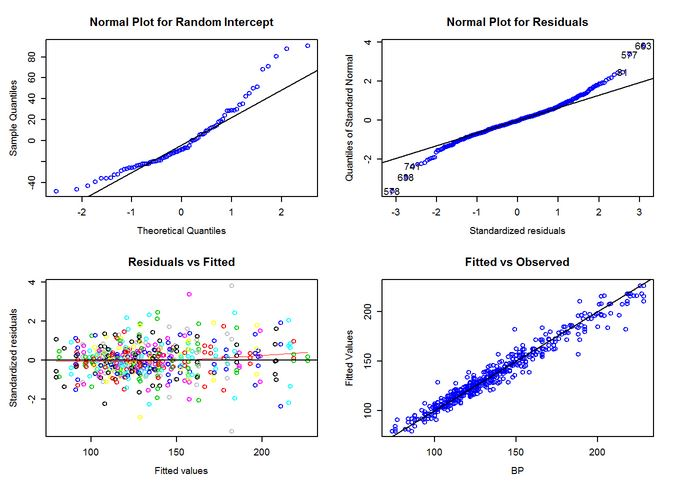
\includegraphics[width=0.9\linewidth]{images/ResidPlot}
		\caption{}
		\label{fig:ResidPlot}
	\end{figure}


	
	
	%------------------------------------------------------------%
	\subsubsection{Residuals in the Blood Data Example}
	The fitted model used in the Blood data example, \texttt{JS.ARoy20091}, was fitted using the \texttt{lme()} function from the nlme package, and as such, is stored as an \texttt{lme} object. The \texttt{residual} functions extracts residuals of a fitted LME model, depending on the type of residual required.
	
	\begin{figure}[h!]
		\centering
		\includegraphics[width=0.9\linewidth]{images/Residuals-JS-roy}
		\caption{}
		\label{fig:Residuals-JS-ARoy2009}
	\end{figure}
	
	\subsubsection{Summary of Paper}
	%Summary of Schabenberger
	Standard residual and influence diagnostics for linear models can be extended to LME models.
	The dependence of the fixed effects solutions on the covariance parameters has important ramifications on the perturbation analysis.	
	Calculating the studentized residuals-And influence statistics whereas each software procedure can calculate both conditional and marginal raw residuals, only SAs Proc Mixed is currently the only program that provide studentized residuals Which ave preferred for model diagnostics. The conditional Raw residuals ave not well suited to detecting outliers as are the studentized conditional residuals. (schabenbege r)
	
	
	LME are flexible tools for the analysis of clustered and repeated measurement data. LME extend the capabilities of standard linear models by allowing unbalanced and missing data, as long as the missing data are MAR. Structured covariance matrices for both the random effects G and the residuals R. missing at Random.
	
	A conditional residual is the difference between the observed valve and the predicted valve of a dependent variable- Influence diagnostics are formal techniques that allow the identification observation that heavily influence estimates of parameters.
	To alleviate the problems with the interpretation of conditional residuals that may have unequal variances, we consider sealing.
	Residuals obtained in this manner ave called studentized residuals.
	
	\begin{itemize}
		\item Standard residual and influence diagnostics for linear models can be extended to linear mixed models. The dependence of fixed-effects solutions on the covariance parameter estimates has important ramifications in perturbation analysis. 
		\item To gauge the full impact of a set of observations on the analysis, covariance parameters need to be updated, which requires refitting of the model. 
		%	\item The experimental INFLUENCE option of the MODEL statement in the MIXED procedure (SAS 9.1) enables you to perform iterative and noniterative influence analysis for individual observations and sets of observations.
		
		\item The conditional (subject-specific) and marginal (population-averaged) formulations in the linear mixed model enable you to consider conditional residuals that use the estimated BLUPs of the random effects, and marginal residuals which are deviations from the overall mean. 
		\item Residuals using the BLUPs are useful to diagnose whether the random effects components in the model are specified correctly, marginal residuals are useful to diagnose the fixed-effects components. 
		\item Both types of residuals are available in SAS 9.1 as an experimental option of the MODEL statement in the MIXED procedure.
		
		\item It is important to note that influence analyses are performed under the assumption that the chosen model is correct. Changing the model structure can alter the conclusions. Many other variance models have been fit to the data presented in the repeated measures example. You need to see the conclusions about which model component is affected in light of the model being fit.
		%	\item  For example, modeling these data with a random intercept and random slope for each child or an unstructured covariance matrix will affect your conclusions about which children are influential on the analysis and how this influence manifests itself.
	\end{itemize}
	
	
	\bibliography{DB-txfrbib}
	
	
\end{document}


%---------------------------------------------------------------------------------------------------%


